\section{CTA-Pipelining as a Scaling Method: Comparing against Micro-batching and TP} 

In this section, we demonstrate how CTA-pipelining can be used as a latency-oriented spatial scaling method, on optimizing single batch execution latency. The evaluation consists of two parts. First, we perform a comparison against traditional static micro-batch chunk pipelining (also known as micro-batching), using a multi-layer GEMM as the primary workload. Second, we compare CTA-pipelining against Tensor Parallelism (TP), and demonstrate how it can be combined with TP by evaluating performance across different scaling setups and input sizes.

The workload chosen for this section consists of multi-layer GEMM operations, which simulate LLM MLP layers by omitting intermediate element-wise non-linear activations for simplicity. This abstraction assigns specific meanings to our matrix dimensions. For example, in the two-layer GEMM $Y=XAB$, $X$ represents the input activation tensor, while $A$ and $B$ are the respective weight matrices. Because of this mapping, we fix the weight matrices $A$ and $B$ at 8192 by 8192 to reflect typical LLM architectures, while leaving the row dimension of $X$ flexible for varying input sequence lengths. As before, the input and output data types are set to BF16, and the Tensor Core accumulator type is set to FP32, with specific CUTLASS configuration determined by the CUTLASS profiler. 

Our testbeds is an 8-GPU NVIDIA B200 system with $5^{th}$ generation NVLink. All the CTA-pipelining implementation utilize the integration with SM100 TMA Warp Specialized kernel introduced in previous section. The baseline we compare against are built using state-of-the-art cuBLAS~\cite{cublas} and NCCL~\cite{nccl} libraries. All execution time we present are the average of 5 repeated runs, where data are collected using NVIDIA Nsight Systems~\cite{nsight}. 

\subsection{Comparison Against Micro-Batch Chunk Pipelining}

Intuitively, the CTA-pipelining execution model is similar to micro-batching operating at the finest granularity. However, they are architecturally different, especially in terms of kernel efficiency and parallelism. Unlike traditional methods, CTA-pipelining does not explicitly pre-partition the input into static chunks, nor does it invoke multiple separate kernel launches for each stage of the pipeline. Instead, it preserves the original kernel structure and leverages the unified memory space within the NVLink domain for coordination. This approach preserves single-kernel efficiency while enabling cross-device parallelism, qualifying it as a general, latency-oriented spatial scaling method. In this subsection, we present experimental results that support these claims.

To compare against static micro-batching, we performed experiments running a multi-layer GEMM workload across multiple GPUs using our prototype built with NVIDIA CUTLASS. As a baseline, static micro-batching is built with the NVIDIA cuBLAS library. For this specific scenario, cuBLAS is considered a stronger baseline than CUTLASS, as it self-adapts to different input sizes, providing the most robust comparison when varying static chunk sizes. Furthermore, the baseline is executed using CUDA Graph to minimize kernel launching overhead. 

For demonstration, the input sequence length is chosen to be 16384, while the weight dimensions are fixed to be 8192 by 8192, as introduced before. Each GPU is assigned one layer of the GEMM workload, and increasing number of GPUs also increases the layer of GEMM operations. Micro-batching is performed by splitting the input matrix in row-major order, where the "chunk size" we refer to is the input sequence length (row dimension) of the split sub-matrix, and the number of pipeline stages is equal to the number of GEMM layers. This experimental setup is illustrated in Figure~\ref{fig:chunk-experiment}. 

\begin{figure}[htbp]
    \centering
    
    \begin{subfigure}[b]{0.9\columnwidth}
        \centering
        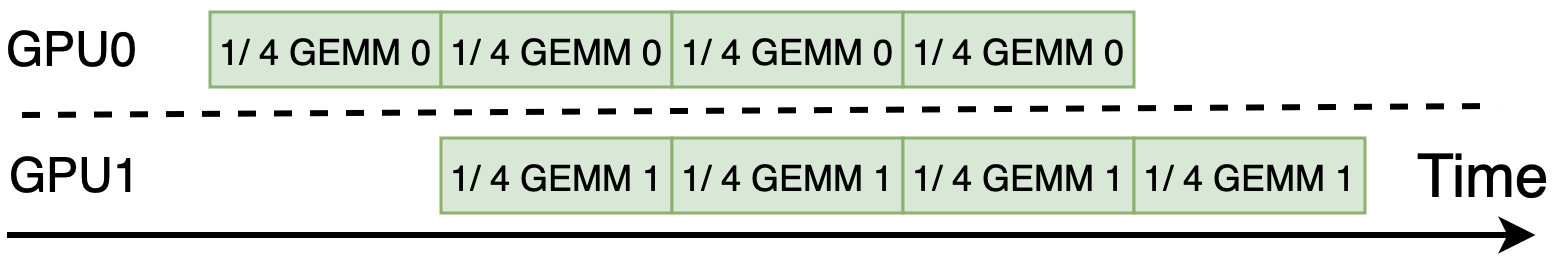
\includegraphics[width=\columnwidth]{fig/chunk-basic.png}
        \caption{}
        \label{fig:chunk-basic}
    \end{subfigure}

    \begin{subfigure}[b]{0.9\columnwidth}
        \centering
        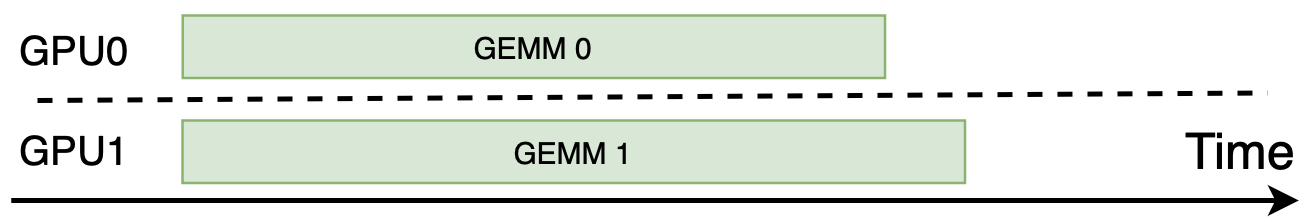
\includegraphics[width=\columnwidth]{fig/chunk-cta.png}
        \caption{}
        \label{fig:chunk-cta}
    \end{subfigure}
    
    \caption{The experiment setup for comparing executing multiple layers of GEMM with (a) micro-batch chunk pipelining, and (b) CTA-pipelining, using GPU=2 as an example.}
    \label{fig:chunk-experiment}

\end{figure}


\begin{figure}[t]
    
    \begin{subfigure}[b]{\columnwidth}
        \centering
        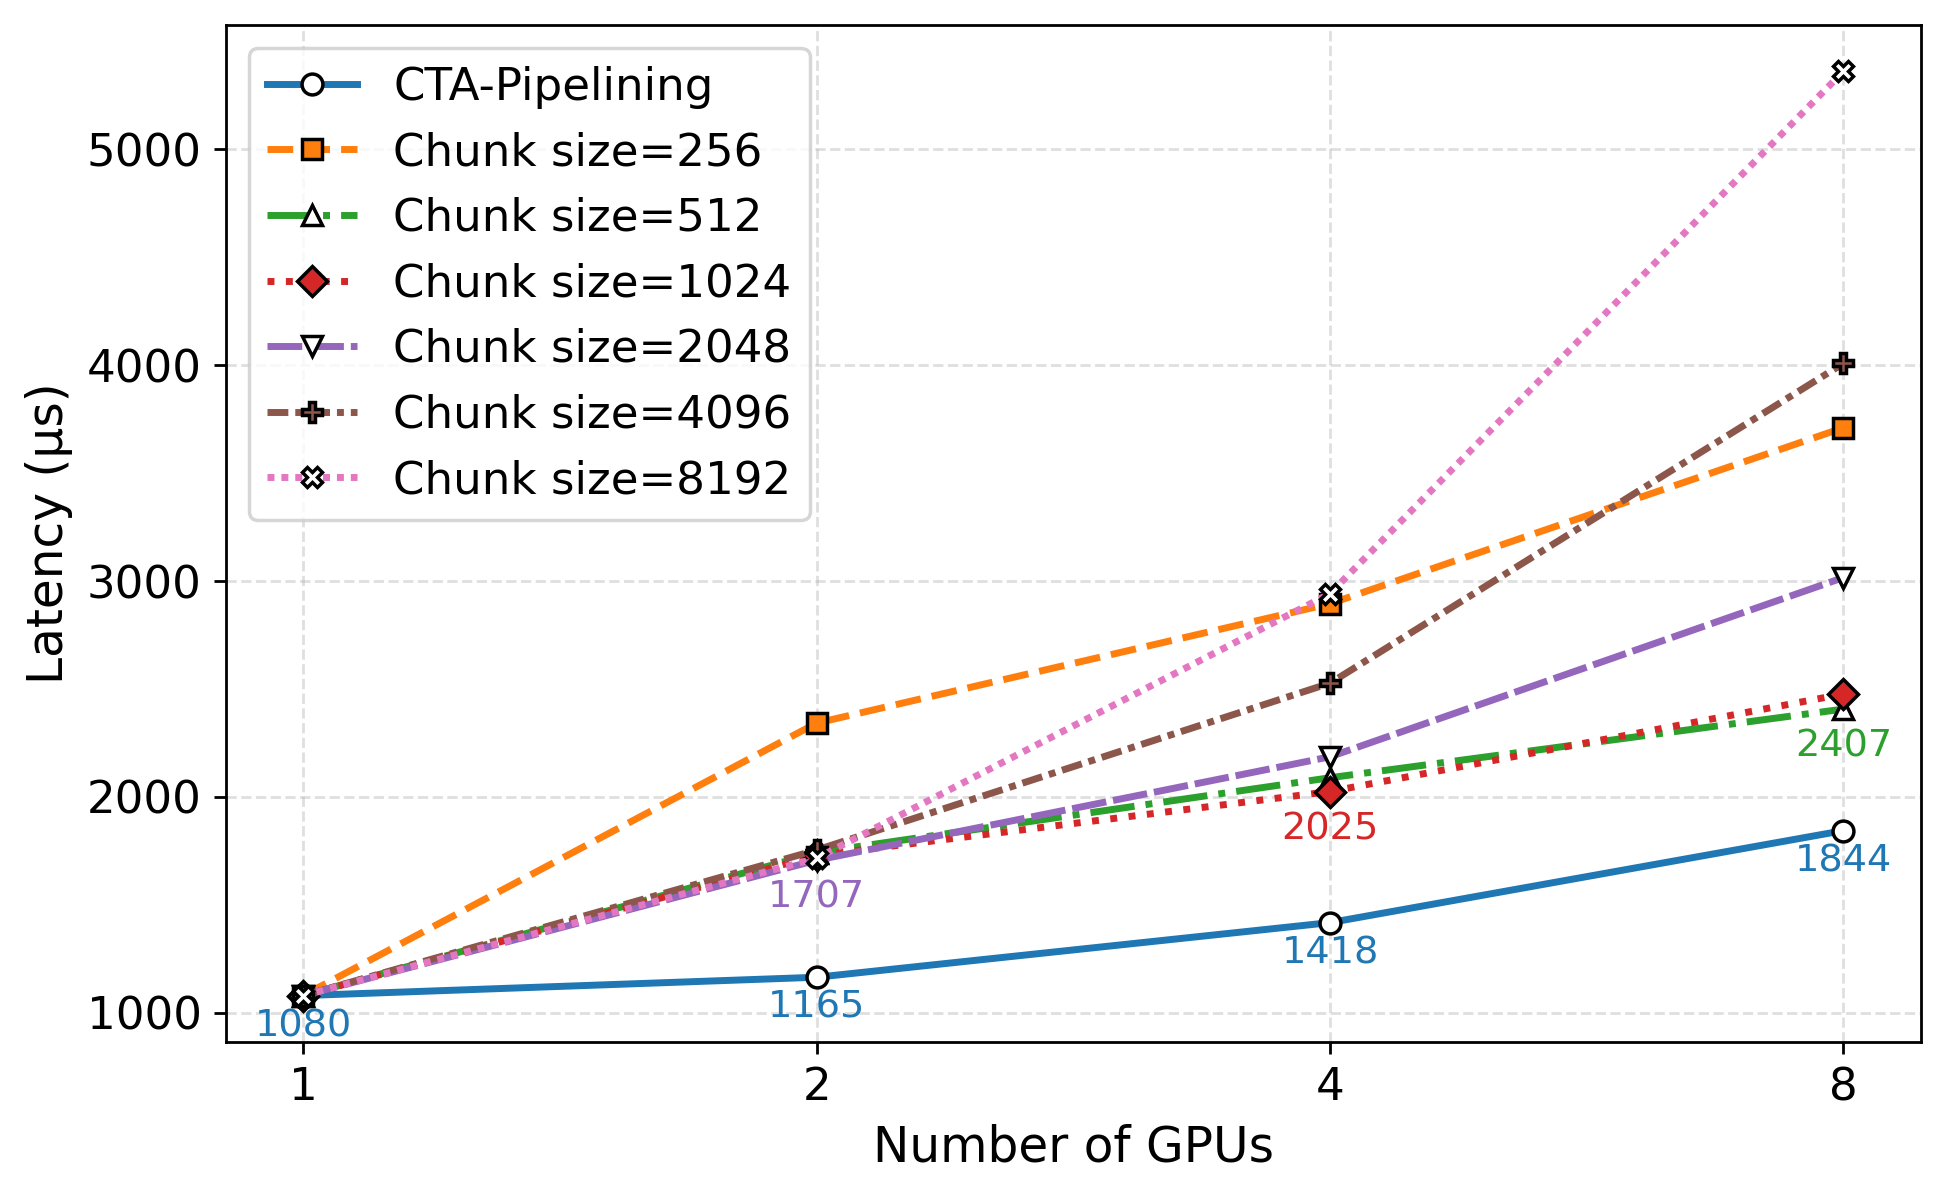
\includegraphics[width=\columnwidth]{fig/chunk_latency.png}
    \end{subfigure}
    
    \begin{subfigure}[b]{\columnwidth}
        \centering
        \small
        \begin{tabular}{|c|c|c|c|c|}
            \hline
            Number of GPUs & 1 & 2 & 4 & 8 \\
            \hline
            % Micro-batching ($\mu$s) & 1080 & 1707 & 2025 & 2407 \\ 
            % \hline
            % CTA-Pipelining ($\mu$s) & 1080 & 1165 & 1418 & 1844 \\ 
            % \hline
            Latency Reduction & - & 31.8\% & 30.0\% & 23.4\% \\ 
            \hline
        \end{tabular}
    \end{subfigure}
    
    \caption{Multi-layer GEMM (16384$\times$8192$\times$8192) latency reduction, comparing CTA-pipelining against micro-batching implemented with cuBLAS. The number of GEMM layers increases with the number of GPUs.}
    \label{fig:chunk-speedup}

    \vspace{-3mm}

\end{figure}

The experimental results are presented in Figure~\ref{fig:chunk-speedup}. We compare CTA-pipelining against static micro-batching across varying numbers of GPUs and a range of chunk sizes. As optimal chunk size selection is critical for the baseline's performance, sweeping this parameter ensures a fair comparison. The results demonstrate that CTA-pipelining consistently outperforms static micro-batching across all evaluated configurations. Comparing against the optimal chunk size in the sweeping, CTA-pipelining reduces latency by 31.8\%, 30.0\%, and 23.4\% in 2, 4, and 8 GPU setup, respectively. The more common 2-layer GEMM case, representing MLP layers, is further evaluated across different input sequence length in Figure~\ref{fig:2-layer}, further proving CTA-pipelining's effectiveness.

The fundamental problem with traditional micro-batch chunk pipelining can be viewed as a dilemma between parallelism and kernel efficiency when selecting chunk sizes. When the chunk size is too large, the head and tail phases of the pipeline execution become longer, where most devices waiting for the previous pipeline stage to finish, thereby decreasing overall parallelism. If the chunk size is too small, the compute efficiency of the individual kernels suffers. GPU kernels require sufficiently large input sizes to maintain high hardware utilization, and small kernels often suffer from quantization effects. Smaller chunk sizes also implies larger number of kernel launches, accumulating more kernel launching bubbles. 

In contrast, CTA-pipelining achieves overlap at the finest possible granularity: the CTA level. At the same time, as it does not explicitly split the input into discrete chunks, the original compute efficiency of the kernel is preserved. This effectively solves the traditional chunking dilemma. 

Furthermore, executing micro-batching as a spatially across devices introduces additional overhead. It suffers not only from pipeline bubbles induced by repeated kernel launches, but also from cross-device write latency, as the final wave of TMA writes must post before the kernel can terminate. In contrast, our execution trace analysis in Figure~\ref{fig:pic-warp} demonstrates that, while CTA-pipelining requires a system-wide memory fence to guarantee inter-device memory consistency, the warp-specialized kernel design effectively hides this overhead. 

Despite its significant benefits, CTA-pipelining does become less effective at extremely small input sizes. As shown in Figure~\ref{fig:2-layer}, while protocol overhead is mostly hidden, it does stand out when kernel execution time drops to the 100$\mu$s range (e.g., sequence length 1024). In the most extreme case, where a kernel requiring only a single wave of CTAs, intra-kernel pipelining becomes physically impossible. Nevertheless, traditional micro-batching is also reaching its limit under such extreme scenarios.

In summary, CTA-pipelining is a superior method than micro-batch chunk pipelining in most of the cases. It maximizes cross-device parallelism and preserves native kernel efficiency, while effectively hiding pipeline bubbles and global memory fence overheads. As an added practical benefit, the CTA-pipelining approach saves the tuning effort typically required to discover the optimal micro-batch chunk size. For workflows that already utilize micro-batch pipelining executing, CTA-pipelining can serve as a direct replacement. 


\begin{figure}[t]

    \begin{subfigure}[b]{\columnwidth}
        \centering
        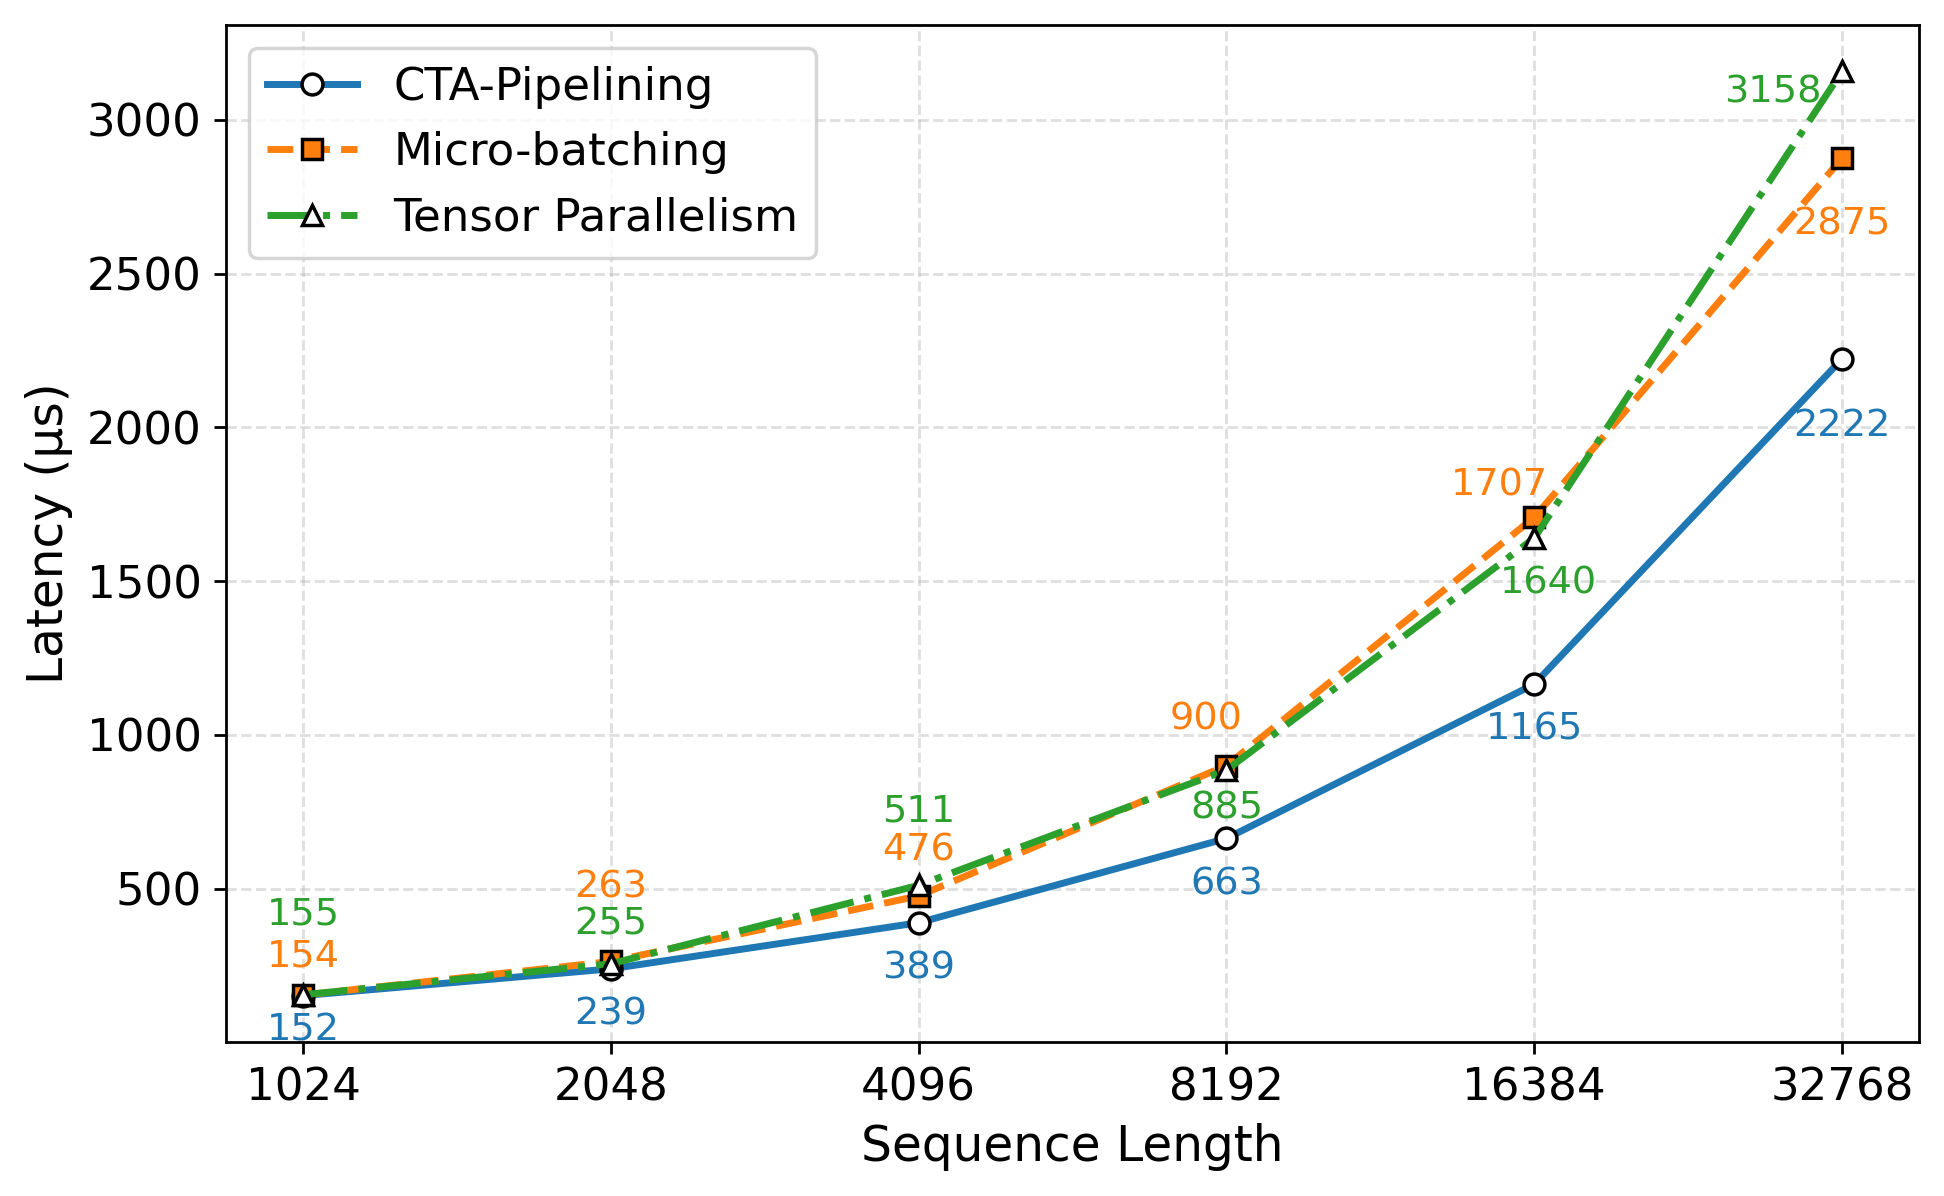
\includegraphics[width=\columnwidth]{fig/chunk_tp_latency.png}
    \end{subfigure}
    
    \begin{subfigure}[b]{\columnwidth}
        \centering
        \small
        
        \begin{tabular}{|c|c|c|c|c|c|c|}
            \hline
            \textbf{Input} & \textbf{1024} & \textbf{2048} & \textbf{4096} & \textbf{8192} & \textbf{16384} & \textbf{32768} \\
            % Input & 1024 & 2048 & 4096 & 8192 & 16384 & 32768 \\
            \hhline{|=======|}
            % \hline
            % MB ($\mu$s) & 154 & 263 & 476 & 900 & 1707 & 2875 \\ 
            % \hline
            % TP ($\mu$s) & 155 & 255 & 511 & 885 & 1640 & 3158 \\ 
            % \hline
            % CTA ($\mu$s) & 152 & 239 & 389 & 663 & 1165 & 2222 \\ 
            % \hline
            R-MB & 1.3\% & 9.1\% & 18.3\% & 26.3\% & 31.8\% & 22.7\% \\ 
            % against Micro-batching & & & & & & \\
            \hline
            R-TP & 1.9\% & 6.3\% & 23.9\% & 25.1\% & 29.0\% & 29.6\% \\ 
            % against TP & & & & & & \\
            \hline
        \end{tabular}

        \flushleft
        % Input: The input sequence length \\
        % MB: Micro-batching execution latency \\ 
        % TP: Tensor Parallelism execution latency \\
        % CTA: CTA-Pipelining execution latency \\
        R-MB: Latency reduction against micro-batching \\
        R-TP: Latency reduction against Tensor Parallelism \\
        $\ast$ The weight matrices are fixed to be 8192$\times$8192. \\
        $\ast\ast$ The micro-batching execution latency is obtained by sweeping chunk sizes and selecting the optimal one.
    \end{subfigure}

    \caption{CTA-Pipelining latency vs. micro-batching and Tensor Parallelism on 2-layer GEMM, representing MLP layers, on 2 GPUs, across different input sequence length.}
    \label{fig:2-layer}
    \vspace{-3mm}
    
\end{figure}

\subsection{Comparison Against Tensor Parallelism and Integration with Tensor Parallelism for Spatial Scaling}

As discussed in the introduction section, Tensor Parallelism (TP) has emerged as the de facto standard for latency-oriented scaling in multi-GPU environments. We propose CTA-pipelining as an orthogonal spatial scaling technique that can be combined with TP. The evaluation is this section consists of two parts. First, we compare CTA-pipelining against TP on multi-layer GEMM. Second, we evaluates the integration of CTA-pipelining with TP, demonstrating how their combined application can further push the latency optimization frontier.

The baseline TP implementation mirrors the standard Megatron-LM paradigm for LLM MLP layers~\cite{shoeybi2019megatron}. Under standard TP for calculating $Y = XAB$, $A$ is sharded in a column-parallel fashion, and $B$ is sharded in a row-parallel fashion across all participating GPUs. An All-reduce collective operation is then required to sum the partial results. For the pure TP cases, cuBLAS kernels are again used to provide a strong baseline. The NCCL library is used for the All-reduce collective operations.

Note that splitting the input tensor $X$ while replicating the weight matrices $A$ and $B$ across devices to achieve Data Parallelism is not the standard practice for LLM deployments. In modern LLMs, transformer layers are repeated numerous times throughout the architecture, each containing multiple massive MLP weight matrices. As the total parameter size exceeds the memory capacity of a single GPU, replicating these weights across devices is impractical. Instead, weight matrices $A$ and $B$ are sharded across devices, while the input tensor $X$ can be replicated. 


\subsubsection{Comparing CTA-Pipelining Against TP}

% \begin{figure}[tp]
%     \centering

%     \begin{subfigure}[b]{0.9\columnwidth}
%         \centering
%         \includegraphics[width=\columnwidth]{fig/chunk_tp_speedup.png}
%     \end{subfigure}

%     \begin{subfigure}[b]{\columnwidth}
%         \centering
%         \small
%         \begin{tabular}{|c|c|c|c|c|}
%             \hline
%             NUM\_GPU & 1 & 2 & 4 & 8 \\
%             \hline
%             Tensor Parallelism ($\mu$s) & 1080 & 1640 & 2636 & 4493 \\ 
%             \hline
%             CTA-Pipelining ($\mu$s) & 1080 & 1165 & 1418 & 1844 \\ 
%             \hline
%             Latency Reduction & - & 29.0\% & 46.2\% & 59.0\% \\ 
%             \hline
%         \end{tabular}
%     \end{subfigure}

%     \caption{Multi-layer GEMM (16384$\times$8192$\times$8192) speedup and latency reduction, comparing CTA-pipelining against Tensor Parallel, with Micro-batching as a reference. The speedup is against running NUM\_GPU layers of GEMMs sequentially on 1 GPU.}
%     \label{fig:chunk-tp-speedup}

%     \vspace{-3mm}
% \end{figure}

We perform our multi-layer GEMM comparison using the same experimental setup as the micro-batching evaluation above, where the number of GEMM layers increases with the GPU count. Under this setup, following standard Megatron-LM practices, TP requires an All-Reduce operation every two layers. We note that while a 2-layer structure is a more common pattern in real-world workloads, we include one example of multi-layer GEMM here for evaluation completeness. 

\begin{table}
    \centering
    \small
    \caption{Multi-layer GEMM (16384$\times$8192$\times$8192) latency reduction, comparing CTA-pipelining against Tensor Parallelism.}
    \label{tab:tp-speedup}
    \begin{tabular}{|c|c|c|c|c|}
        \hline
        Number of GPUs & 1 & 2 & 4 & 8 \\
        \hline
        Tensor Parallelism ($\mu$s) & 1080 & 1640 & 2636 & 4493 \\ 
        \hline
        CTA-Pipelining ($\mu$s) & 1080 & 1165 & 1418 & 1844 \\ 
        \hline
        Latency Reduction & - & 29.0\% & 46.2\% & 59.0\% \\ 
        \hline
    \end{tabular}
    \vspace{-3mm}
\end{table} 

The experiment results are shown in Table~\ref{tab:tp-speedup}. CTA-pipelining effectively reduces multi-layer GEMM latency by 29.0\%, 46.2\%, and 59.0\% on 2, 4, and 8 GPUs, respectively. The primary source of this benefit is that, within this setup, CTA-pipelining completely avoids All-Reduce communication. Conversely, TP requires frequent communication for every two layers. This demonstrates the advantage of using CTA-pipelining as a scaling method for suitable workflows that can execute in pure CTA-pipelining manner end-to-end.

As 2-layer GEMM represents a more realistic setup, similarly, we provide further evaluation across different input sequence length in Figure~\ref{fig:2-layer}. Result demonstrates the general benefit of CTA-pipelining against TP by saving communication time, despite the limitation on extremely small input sizes, which has been discussed in previous subsection. 

\begin{figure}[bp]
    \centering
    
    \begin{subfigure}[b]{0.9\columnwidth}
        \centering
        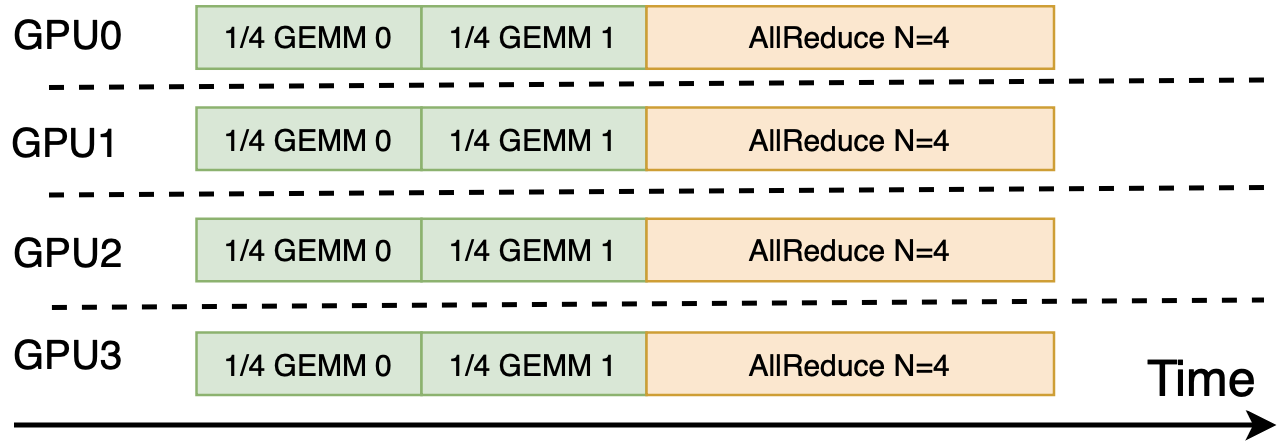
\includegraphics[width=\columnwidth]{fig/tp-basic.png}
        \caption{}
        \label{fig:tp-basic}
    \end{subfigure}

    \begin{subfigure}[b]{0.9\columnwidth}
        \centering
        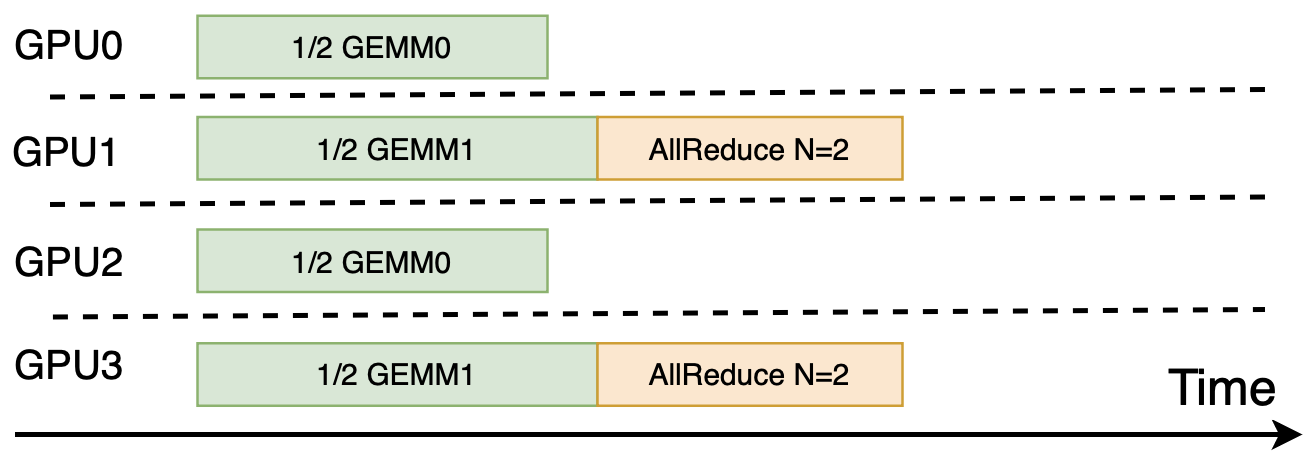
\includegraphics[width=\columnwidth]{fig/tp-cta.png}
        \caption{}
        \label{fig:tp-cta}
    \end{subfigure}
    
    \caption{The experiment setup for comparing executing 2 Layers of GEMM using (a) pure TP, and (b) the combination of TP and CTA-pipelining, using GPU=4 as an example.}
    \label{fig:tp-experiment}

    \vspace{-3mm}

\end{figure}

\begin{figure*}[htbp]
    \centering
    
    \begin{subfigure}[b]{0.32\textwidth}
        \centering
        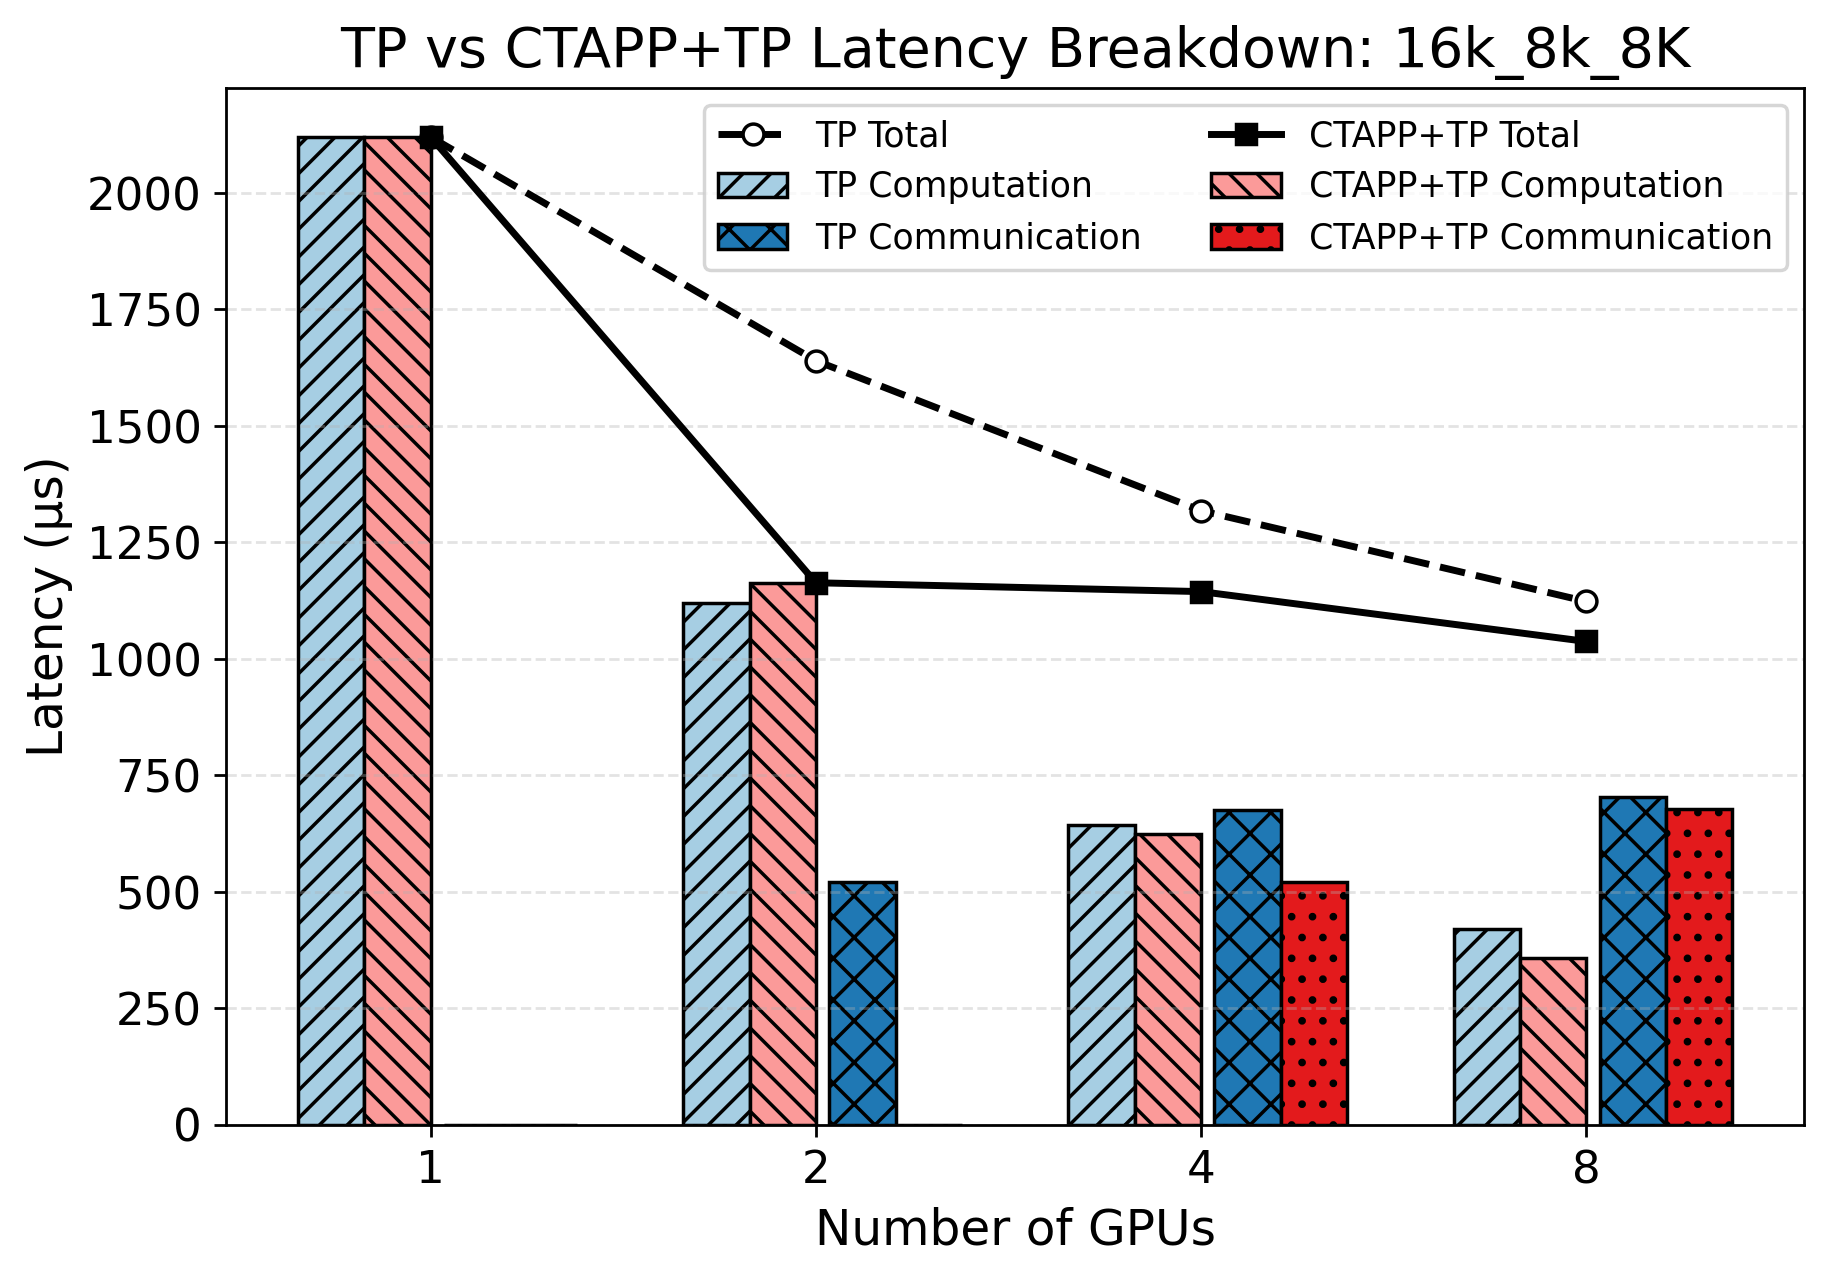
\includegraphics[width=\textwidth]{fig/tp_16k_8k_8K.png}
        \caption{}
        \label{fig:tp-16k}
    \end{subfigure}
    \begin{subfigure}[b]{0.32\textwidth}
        \centering
        \includegraphics[width=\textwidth]{fig/tp_8k_8k_8K.png}
        \caption{}
        \label{fig:tp-8k}
    \end{subfigure}
    \begin{subfigure}[b]{0.32\textwidth}
        \centering
        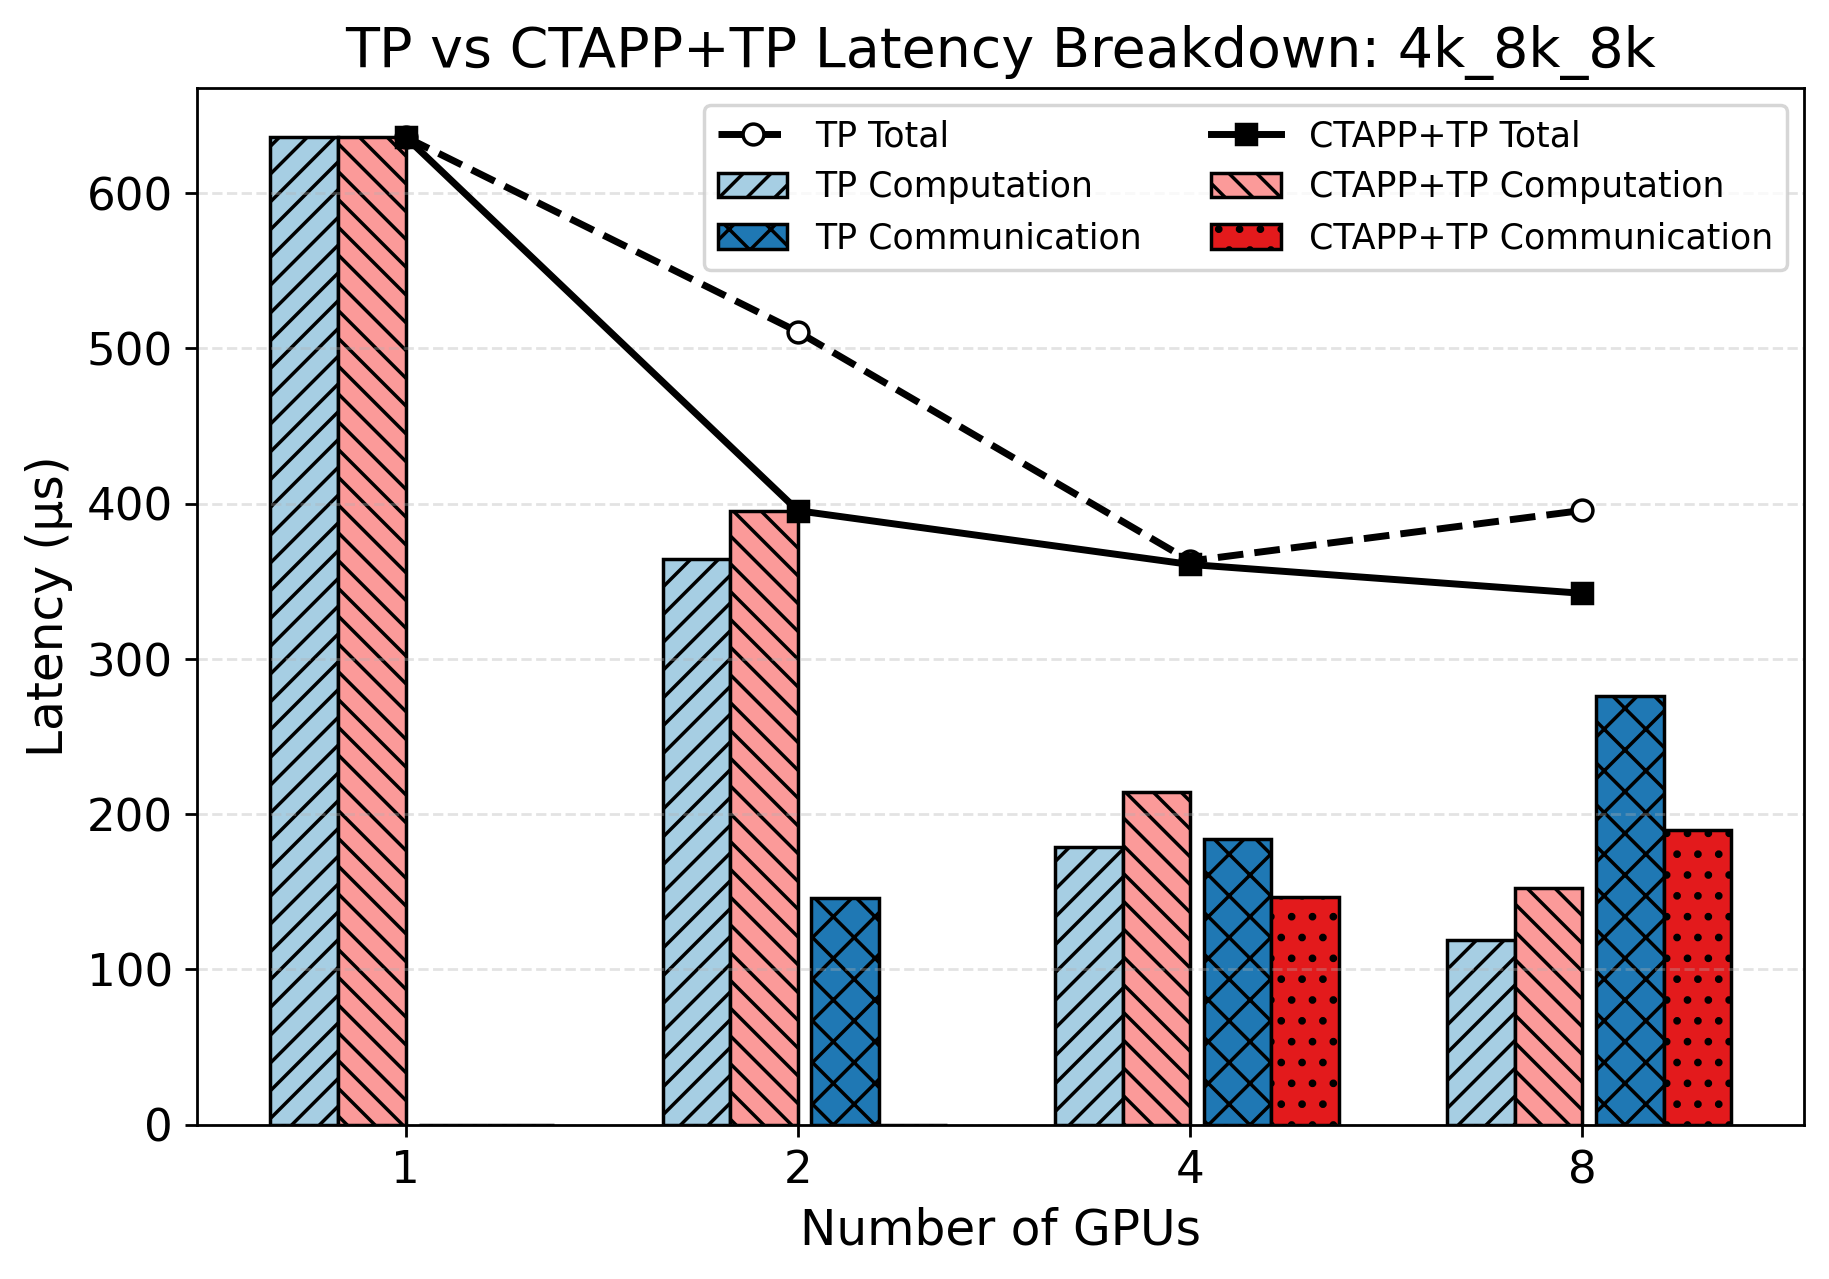
\includegraphics[width=\textwidth]{fig/tp_4k_8k_8k.png}
        \caption{}
        \label{fig:tp-4k}
    \end{subfigure}

    \caption{The execution latency breakdown of 2-layer GEMM with different input sequence lengths, comparing pure TP and the combination of TP and CTA-pipelining.}
    \label{fig:tp-result}

    \vspace{-4mm}

\end{figure*}

\subsubsection{Combining CTA-pipelining with TP}

As demonstrated above, while CTA-pipelining provides significant benefits when workflows can execute entirely within this paradigm, some workflows lack enough kernels to form sufficient pipeline stages across multiple GPUs. In such scenarios, we purpose that, CTA-pipelining can be combined with TP as an orthogonal scaling dimension to further reduce latency. We demonstrate this capability using 2-layer GEMMs, representing the MLP layers.

To integrate CTA-pipelining with TP, we alter this sharding strategy. Rather than distributing $A$ and $B$ across all devices, we partition the hardware into 2-GPU groups. The weight matrices are then sharded evenly across these groups. Within any given group, the paired GPUs utilize CTA-pipelining to execute the local two-layer GEMM ($Y_i = XA_iB_i$). In this setup, the number of ranks involved in the final All-reduce operation is equal to the number of groups, halving the collective communication world size compared to the pure TP case. Figure~\ref{fig:tp-experiment} provides an example comparing pure TP with this combined CTA-pipelining and TP approach.

As described before, the weight matrices are fixed to be 8192 by 8192. We vary the input sequence length across 4096, 8192, and 16384 as representative user workload sizes. 

The results are shown in Figure~\ref{fig:tp-result}, with the lines showing the trend of total execution latency, and bars explicitly separate the computation and communication times for each setup. These results demonstrate that combining CTA-pipelining with TP provides a beneficial deployment strategy for multi-GPU scenarios, by pushing the latency frontier even further compared to pure TP deployment. 

The most direct benefit comes from the reduction in the world size involved in the All-reduce operation, which directly reduces the overall communication time. In some cases, such as in Figure~\ref{fig:tp-4k}, increasing pure TP degree can result in negative impact, since the communication time dominates, while combining with CTA-pipelining continues the latency reduction with more GPU resources. 

The other factor to consider is the pure computation time. When the TP degree is large, the input size per GPU becomes small, which can degrade kernel efficiency, similar to the micro-batching discussed earlier. By integrating CTA-pipelining, we effectively reduce the required TP degree, preserves larger matrix dimensions, and thereby benefits compute efficiency. However, executing via CTA-pipelining introduces additional pipeline's ramp-up delay (the one-wave CTA execution latency), which counteracts some of these computational gains. As a result, whether the computation time get benefit from combining with CTA-pipelining varies across different matrix sizes. 

In summary, the above experiments demonstrates that CTA-pipelining is a qualified spatial scaling method that is orthogonal to TP, allowing it to be seamlessly combined with TP for multi-GPU deployments. Compared to pure TP, this combined approach provides clear communication benefits, along with computational benefits in certain scenarios. Ultimately, this provides a powerful alternative for deploying multi-GPU workloads and holds the potential to further scale applications for lower latency, particularly when the whole workload can be executed in pure CTA-pipelining manner.
